%load any "/usepackage" here...
\documentclass{pnastwo}

%% ADDITIONAL OPTIONAL STYLE FILES Font specification

%\usepackage{PNASTWOF}
\usepackage[version=3]{mhchem}
\usepackage[round,numbers,sort&compress]{natbib}
\usepackage{fixltx2e}
\usepackage{booktabs}
\usepackage{multirow}
\usepackage{tablefootnote}

\bibpunct{(}{)}{,}{n}{,}{,}
\bibliographystyle{pnas2011}

\renewcommand{\thefigure}{S\arabic{figure}}
\renewcommand{\thetable}{S\arabic{table}}
\renewcommand{\theequation}{S\arabic{equation}}
\renewcommand{\thesection}{S\arabic{section}}

%% OPTIONAL MACRO DEFINITIONS
\def\s{\sigma}
%%%%%%%%%%%%
%% For PNAS Only:
%\url{www.pnas.org/cgi/doi/10.1073/pnas.0709640104}
\copyrightyear{2014}
\issuedate{Issue Date}
\volume{Volume}
\issuenumber{Issue Number}
%\setcounter{page}{2687} %Set page number here if desired
%%%%%%%%%%%%

\begin{document}

\title{Supporting Information for: \\
The different facets of ice have different hydrophilicities: Friction at water /
  ice-I\textsubscript{h} interfaces}

\author{Patrick B. Louden\affil{1}{Department of Chemistry and Biochemistry, University of Notre Dame, Notre Dame,
IN 46556}
\and
J. Daniel Gezelter\affil{1}{}}

\contributor{Submitted to Proceedings of the National Academy of Sciences
of the United States of America}

\maketitle

\begin{article}

\section{Overview}
The supporting information contains further details about the model
construction, analysis methods, and supplies figures that support the
data presented in the main text.

\section{Construction of the Ice / Water interfaces}
Ice I$_\mathrm{h}$ crystallizes in the hexagonal space group
P$6_3/mmc$, and common ice crystals form hexagonal plates with the
basal face, $\{0~0~0~1\}$, forming the top and bottom of each plate, and
the prismatic facet, $\{1~0~\bar{1}~0\}$, forming the sides.  In extreme
temperatures or low water saturation conditions, ice crystals can
easily form as hollow columns, needles and dendrites. These are
structures that expose other crystalline facets of the ice to the
surroundings.  Among the more common facets are the secondary prism,
$\{1~1~\bar{2}~0\}$, and pyramidal, $\{2~0~\bar{2}~1\}$, faces.  

We found it most useful to work with proton-ordered, zero-dipole
crystals that expose strips of dangling H-atoms and lone
pairs~\cite{Buch:2008fk}.  Our structures were created starting from
Structure 6 of Hirsch and Ojam\"{a}e's set of orthorhombic
representations for ice-I$_{h}$~\cite{Hirsch04}.  This crystal
structure was cleaved along the four different facets.  The exposed
face was reoriented normal to the $z$-axis of the simulation cell, and
the structures were extended to form large exposed facets in
rectangular box geometries.  Liquid water boxes were created with
identical dimensions (in $x$ and $y$) as the ice, with a $z$ dimension
of three times that of the ice block, and a density corresponding to 1
g / cm$^3$.  Each of the ice slabs and water boxes were independently
equilibrated at a pressure of 1 atm, and the resulting systems were
merged by carving out any liquid water molecules within 3 \AA\ of any
atoms in the ice slabs.  Each of the combined ice/water systems were
then equilibrated at 225K, which is the liquid-ice coexistence
temperature for SPC/E water~\cite{Bryk02}. Reference
\citealp{Louden13} contains a more detailed explanation of the
construction of similar ice/water interfaces. The resulting dimensions
as well as the number of ice and liquid water molecules contained in
each of these systems are shown in Table S1.

\section{Further details on the shearing (RNEMD) simulations}
All simulations were performed using OpenMD~\cite{OOPSE,openmd}, with a
time step of 2 fs and periodic boundary conditions in all three
dimensions.  Electrostatics were handled using the damped-shifted
force real-space electrostatic kernel~\cite{Ewald}. The systems were
divided into 100 bins along the $z$-axis for the VSS-RNEMD moves,
which were attempted every 2~fs.

The interfaces were equilibrated for a total of 10 ns at equilibrium
conditions before being exposed to either a shear or thermal gradient.
This consisted of 5 ns under a constant temperature (NVT) integrator
set to 225~K followed by 5 ns under a microcanonical (NVE) integrator.
Weak thermal gradients were allowed to develop using the VSS-RNEMD
(NVE) integrator using a small thermal flux ($-2.0\times 10^{-6}$
kcal/mol/\AA$^2$/fs) for a duration of 5 ns to allow the gradient to
stabilize.  The resulting temperature gradient was $\approx$ 10K over
the entire box length, which was sufficient to keep the temperature at
the interface within $\pm 1$ K of the 225~K target.

Velocity gradients were then imposed using the VSS-RNEMD (NVE)
integrator with a range of momentum fluxes. These gradients were
allowed to stabilize for 1~ns before data collection started. Once
established, four successive 0.5~ns runs were performed for each shear
rate.  During these simulations, configurations of the system were
stored every 1~ps, and statistics on the structure and dynamics in
each bin were accumulated throughout the simulations.  Although there
was some small variation in the measured interfacial width between
succcessive runs, no indication of bulk melting or crystallization was
observed.  That is, no large scale changes in the positions of the top
and bottom interfaces occurred during the simulations.

\section{A second method for computing contact angles}
In addition to the spherical cap method outlined in the main text, a
second method for obtaining the contact angle was described by
Ruijter, Blake, and Coninck~\cite{Ruijter99}.  This method uses a
cylindrical averaging of the droplet's density profile.  A threshold
density of 0.5 g cm\textsuperscript{-3} is used to estimate the
location of the edge of the droplet.  The $r$ and $z$-dependence of
the droplet's edge is then fit to a circle, and the contact angle is
computed from the intersection of the fit circle with the $z$-axis
location of the solid surface.  Again, for each stored configuration,
the density profile in a set of annular shells was computed. Due to
large density fluctuations close to the ice, all shells located within
2 \AA\ of the ice surface were left out of the circular fits.  The
height of the solid surface ($z_\mathrm{suface}$) along with the best
fitting origin ($z_\mathrm{droplet}$) and radius
($r_\mathrm{droplet}$) of the droplet can then be used to compute the
contact angle,
\begin{equation}
\theta =  90 + \frac{180}{\pi} \sin^{-1}\left(\frac{z_\mathrm{droplet} -
  z_\mathrm{surface}}{r_\mathrm{droplet}} \right).
\end{equation}

\section{Interfacial widths using structural information}
To determine the structural widths of the interfaces under shear, each
of the systems was divided into 100 bins along the $z$-dimension, and
the local tetrahedral order parameter (Eq. 5 in Reference
\citealp{Louden13}) was time-averaged in each bin for the duration of
the shearing simulation.  The spatial dependence of this order
parameter, $q(z)$, is the tetrahedrality profile of the interface.
The lower panels in figures S2-S5 in the SI show tetrahedrality
profiles (in circles) for each of the four interfaces.  The $q(z)$
function has a range of $(0,1)$, where a value of unity indicates a
perfectly tetrahedral environment.  The $q(z)$ for the bulk liquid was
found to be $\approx~0.77$, while values of $\approx~0.92$ were more
common in the ice. The tetrahedrality profiles were fit using a
hyperbolic tangent function (see Eq. 6 in Reference
\citealp{Louden13}) designed to smoothly fit the bulk to ice
transition while accounting for the weak thermal gradient. In panels
$b$ and $c$ of the same figures, the resulting thermal and velocity
gradients from an imposed kinetic energy and momentum fluxes can be
seen. The vertical dotted lines traversing these figures indicate the
midpoints of the interfaces as determined by the tetrahedrality
profiles.

\section{Interfacial widths using dynamic information}
To determine the dynamic widths of the interfaces under shear, each of
the systems was divided into bins along the $z$-dimension ($\approx$ 3
\AA\ wide) and $C_2(z,t)$ was computed using only those molecules that
were in the bin at the initial time.  To compute these correlation
functions, each of the 0.5 ns simulations was followed by a shorter
200 ps microcanonical (NVE) simulation in which the positions and
orientations of every molecule in the system were recorded every 0.1
ps. 

The time-dependence was fit to a triexponential decay, with three time
constants: $\tau_{short}$, measuring the librational motion of the
water molecules, $\tau_{middle}$, measuring the timescale for breaking
and making of hydrogen bonds, and $\tau_{long}$, corresponding to the
translational motion of the water molecules.  An additional constant
was introduced in the fits to describe molecules in the crystal which
do not experience long-time orientational decay.

In Figures S6-S9, the $z$-coordinate profiles for the three decay
constants, $\tau_{short}$, $\tau_{middle}$, and $\tau_{long}$ for the
different interfaces are shown.  (Figures S6 \& S7 are new results,
and Figures S8 \& S9 are updated plots from Ref \citealp{Louden13}.)
In the liquid regions of all four interfaces, we observe
$\tau_{middle}$ and $\tau_{long}$ to have approximately consistent
values of $3-6$ ps and $30-40$ ps, respectively.  Both of these times
increase in value approaching the interface.  Approaching the
interface, we also observe that $\tau_{short}$ decreases from its
liquid-state value of $72-76$ fs.  The approximate values for the
decay constants and the trends approaching the interface match those
reported previously for the basal and prismatic interfaces.

We have estimated the dynamic interfacial width $d_\mathrm{dyn}$ by
fitting the profiles of all the three orientational time constants
with an exponential decay to the bulk-liquid behavior,
\begin{equation}\label{tauFit}
  \tau(z)\approx\tau_{liquid}+(\tau_{wall}-\tau_{liquid})e^{-(z-z_{wall})/d_\mathrm{dyn}}
\end{equation}
where $\tau_{liquid}$ and $\tau_{wall}$ are the liquid and projected
wall values of the decay constants, $z_{wall}$ is the location of the
interface, as measured by the structural order parameter.  These
values are shown in table 1 in the main text. Because the bins must be
quite wide to obtain reasonable profiles of $C_2(z,t)$, the error
estimates for the dynamic widths of the interface are significantly
larger than for the structural widths.  However, all four interfaces
exhibit dynamic widths that are significantly below 1~nm, and are in
reasonable agreement with the structural width above.

\bibliography{iceWater}
\end{article}

\begin{table}[h]
\centering
\caption{Sizes of the droplet and shearing simulations.  Cell
  dimensions are measured in \AA. \label{tab:method}}
\begin{tabular}{r|cccc|ccccc} 
\toprule
 \multirow{2}{*}{Interface} & \multicolumn{4}{c|}{Droplet} & \multicolumn{5}{c}{Shearing} \\
  & $N_\mathrm{ice}$ & $N_\mathrm{droplet}$ & $L_x$ & $L_y$ & $N_\mathrm{ice}$ & $N_\mathrm{liquid}$ & $L_x$ & $L_y$ & $L_z$  \\ 
\midrule
Basal  $\{0001\}$                    & 12960 & 2048 & 134.70 & 140.04 & 900 & 1846  & 23.87 & 35.83 & 98.64  \\
Pyramidal  $\{2~0~\bar{2}~1\}$       & 11136 & 2048 & 143.75 & 121.41 & 1216 & 2203 & 37.47 & 29.50 & 93.02  \\
Prismatic  $\{1~0~\bar{1}~0\}$       &  9900 & 2048 & 110.04 & 115.00 & 3000 & 5464 & 35.95 & 35.65 & 205.77 \\
Secondary Prism  $\{1~1~\bar{2}~0\}$ & 11520 & 2048 & 146.72 & 124.48 & 3840 & 8176 & 71.87 & 31.66 & 161.55 \\
\bottomrule
\end{tabular}
\end{table}

%S1: contact angle
\begin{figure}
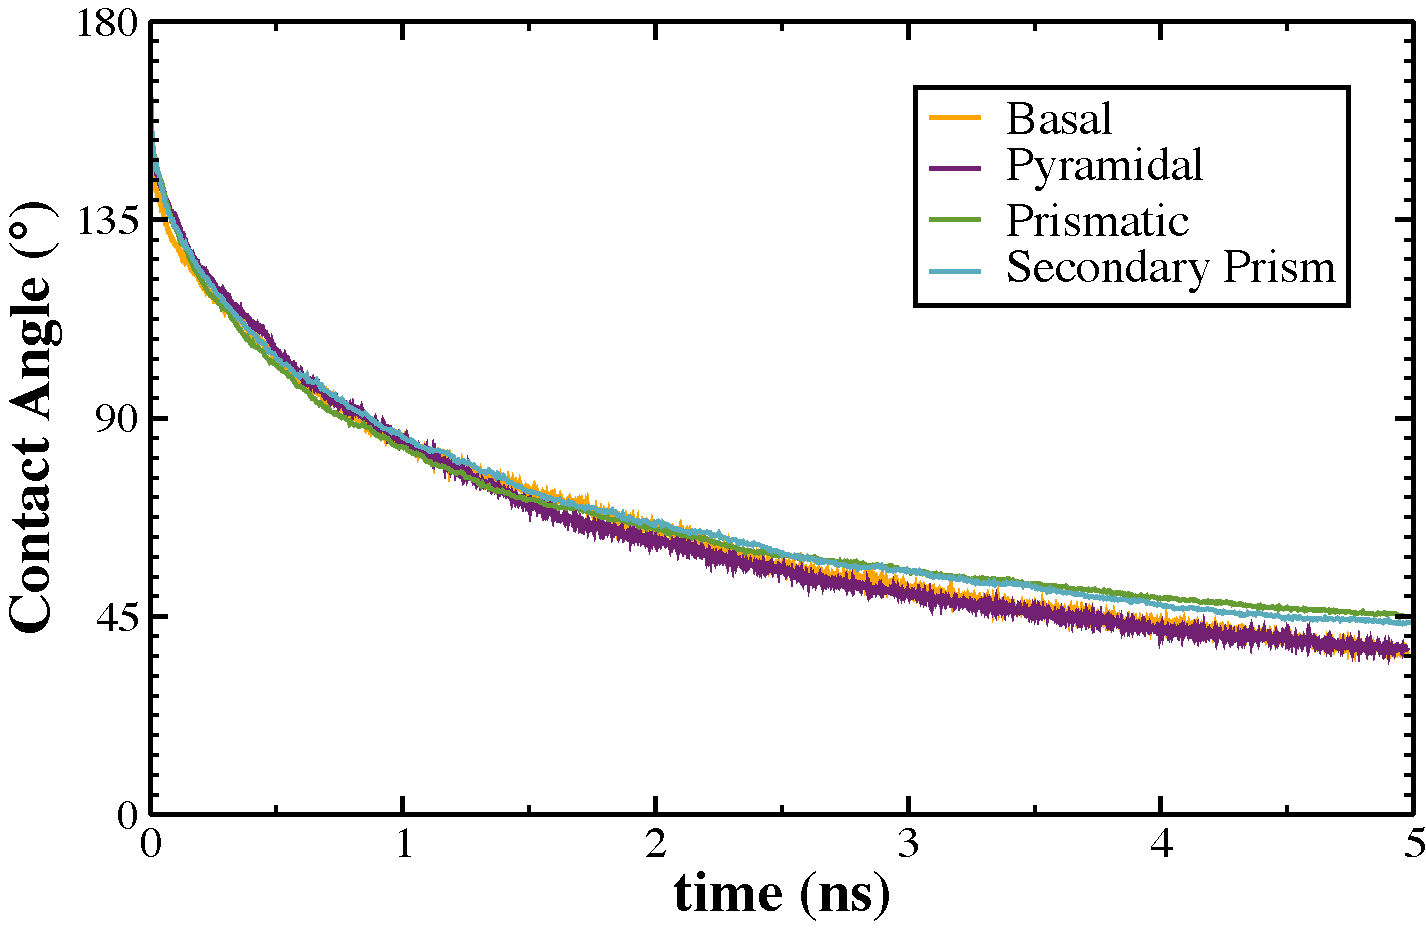
\includegraphics[width=\linewidth]{ContactAngle}
\caption{\label{fig:ContactAngle} The dynamic contact angle of a
  droplet after approaching each of the four ice facets.  The decay to
  an equilibrium contact angle displays similar dynamics.  Although
  all the surfaces are hydrophilic, the long-time behavior stabilizes
  to significantly flatter droplets for the basal and pyramidal
  facets.  This suggests a difference in hydrophilicity for these
  facets compared with the two prismatic facets.}
\end{figure}


%S2-S5 are the z-rnemd profiles
\begin{figure}
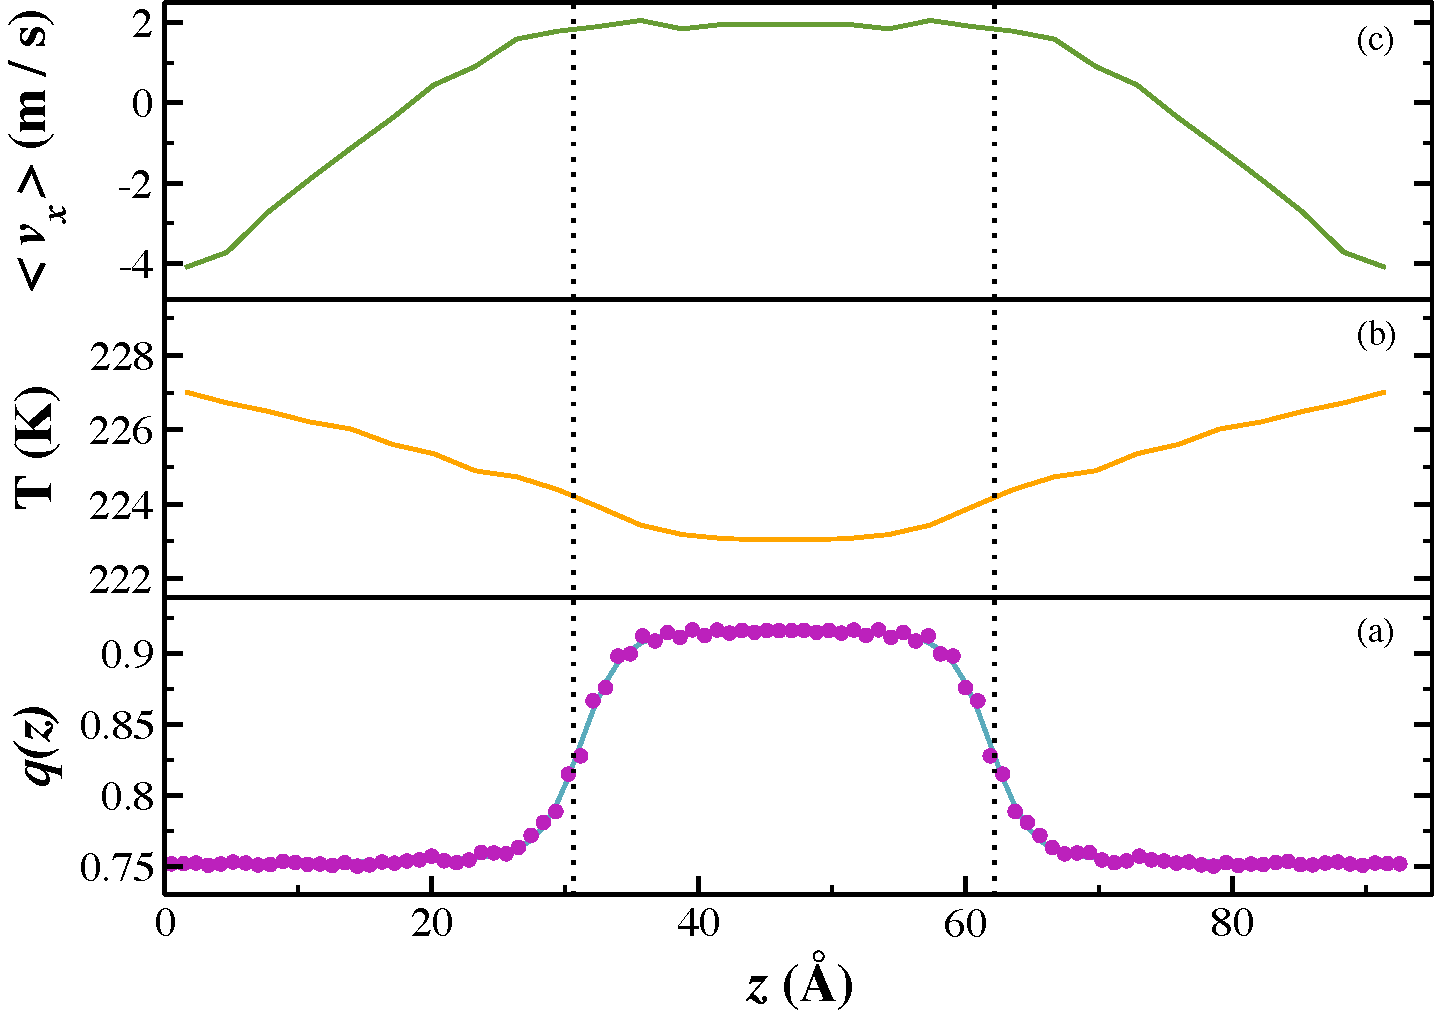
\includegraphics[width=\linewidth]{Pyr_comic_strip}
\caption{\label{fig:pyrComic} Properties of the pyramidal interface
  being sheared through water at 3.8 ms\textsuperscript{-1}. Lower
  panel: the local tetrahedral order parameter, $q(z)$, (circles) and
  the hyperbolic tangent fit (turquoise line).  Middle panel: the
  imposed thermal gradient required to maintain a fixed interfacial
  temperature of 225 K. Upper panel: the transverse velocity gradient
  that develops in response to an imposed momentum flux. The vertical
  dotted lines indicate the locations of the midpoints of the two
  interfaces.}
\end{figure}

\begin{figure}
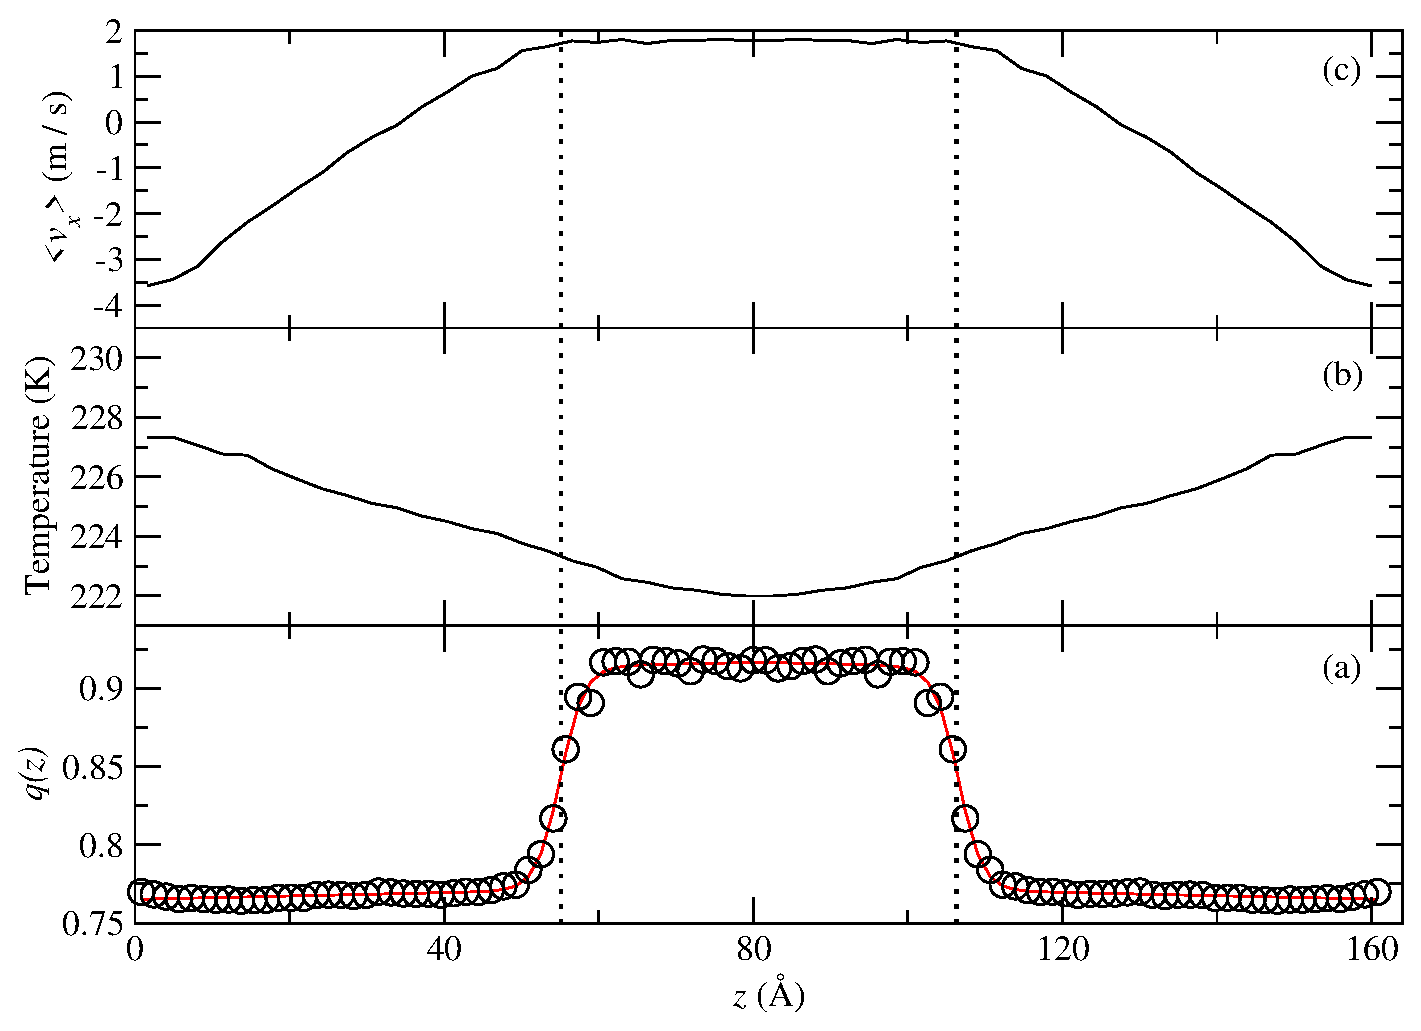
\includegraphics[width=\linewidth]{SP_comic_strip}
\caption{\label{fig:spComic} The secondary prism interface with a shear 
rate of 3.5 \
ms\textsuperscript{-1}. Panel descriptions match those in figure \ref{fig:pyrComic}.}
\end{figure}

\begin{figure}
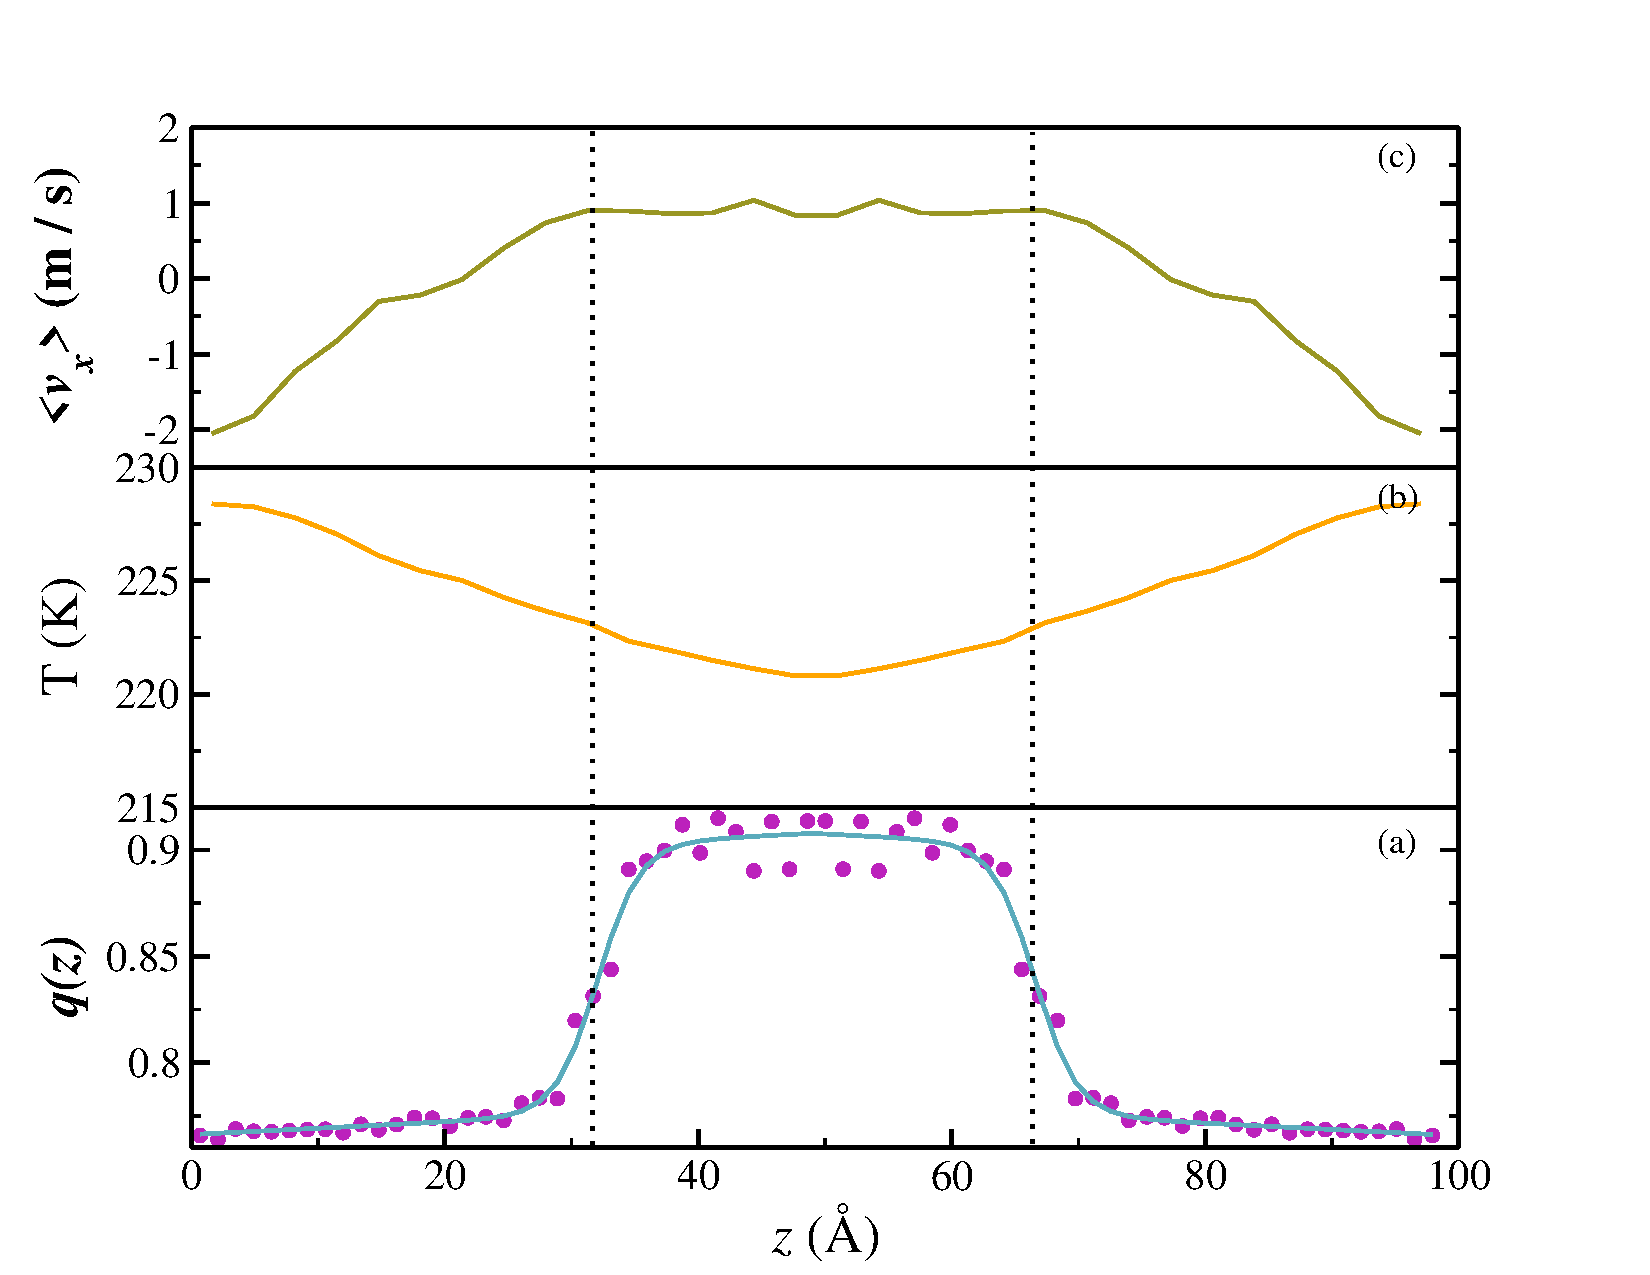
\includegraphics[width=\linewidth]{B_comic_strip}
\caption{\label{fig:bComic} The basal interface with a shear 
rate of 1.3 \
ms\textsuperscript{-1}. Panel descriptions match those in figure \ref{fig:pyrComic}.}
\end{figure}

\begin{figure}
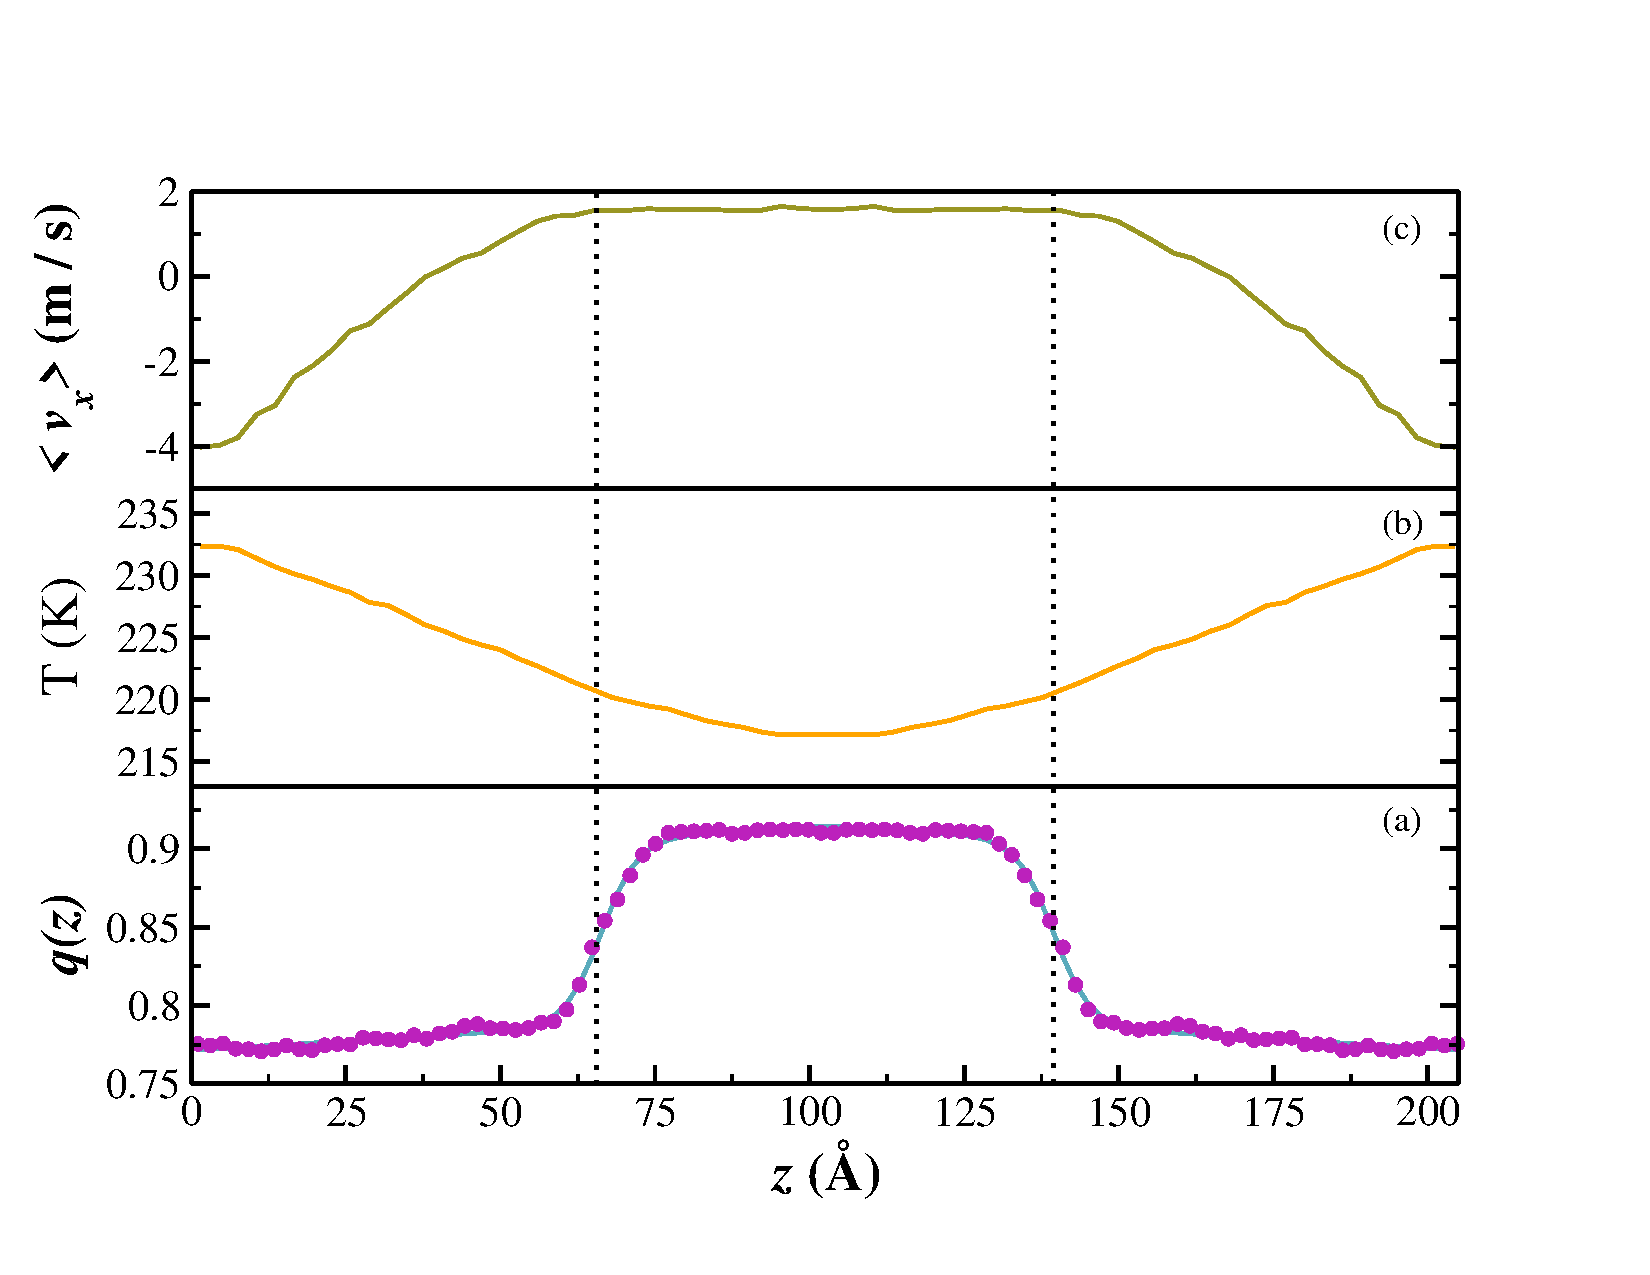
\includegraphics[width=\linewidth]{prismatic_comic_strip}
\caption{\label{fig:pComic} The prismatic interface with a shear 
rate of 2 \
ms\textsuperscript{-1}. Panel descriptions match those in figure \ref{fig:pyrComic}.}
\end{figure}

%Figures S6-S9 are the z-orientation times
\begin{figure}
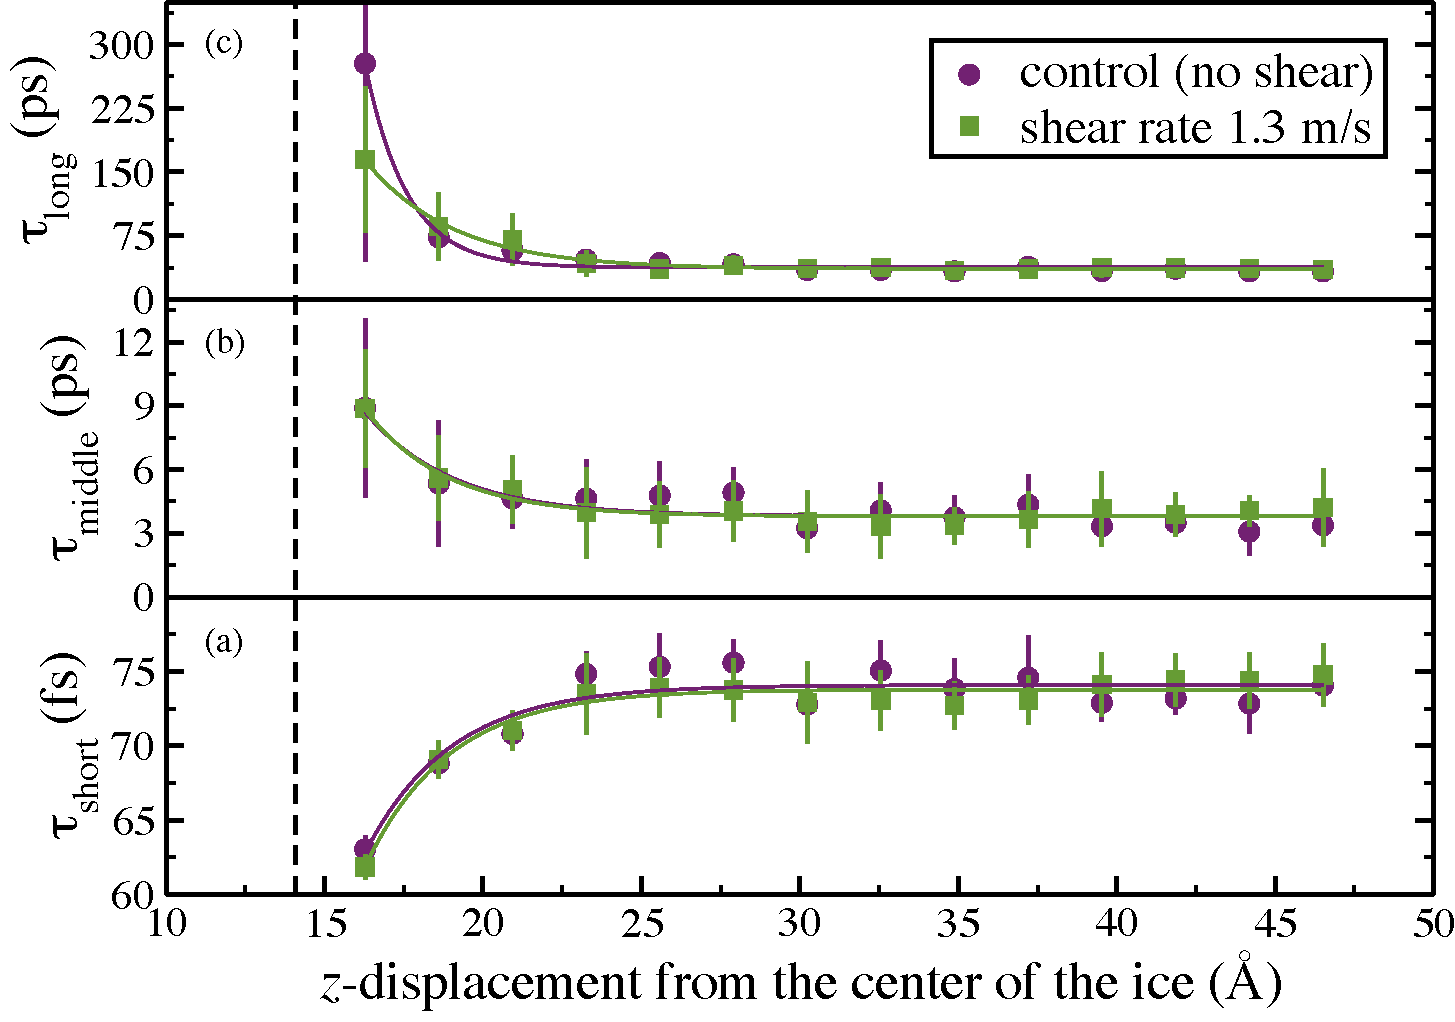
\includegraphics[width=\linewidth]{Pyr-orient}
\caption{\label{fig:PyrOrient} The three decay constants of the
  orientational time correlation function, $C_2(z,t)$, for water as a
  function of distance from the center of the ice slab. The vertical
  dashed line indicates the edge of the pyramidal ice slab determined
  by the local order tetrahedral parameter. The control (circles) and
  sheared (squares) simulations were fit using shifted-exponential
  decay (see Eq. 9 in Ref. \citealp{Louden13}).}
\end{figure}  

\begin{figure}
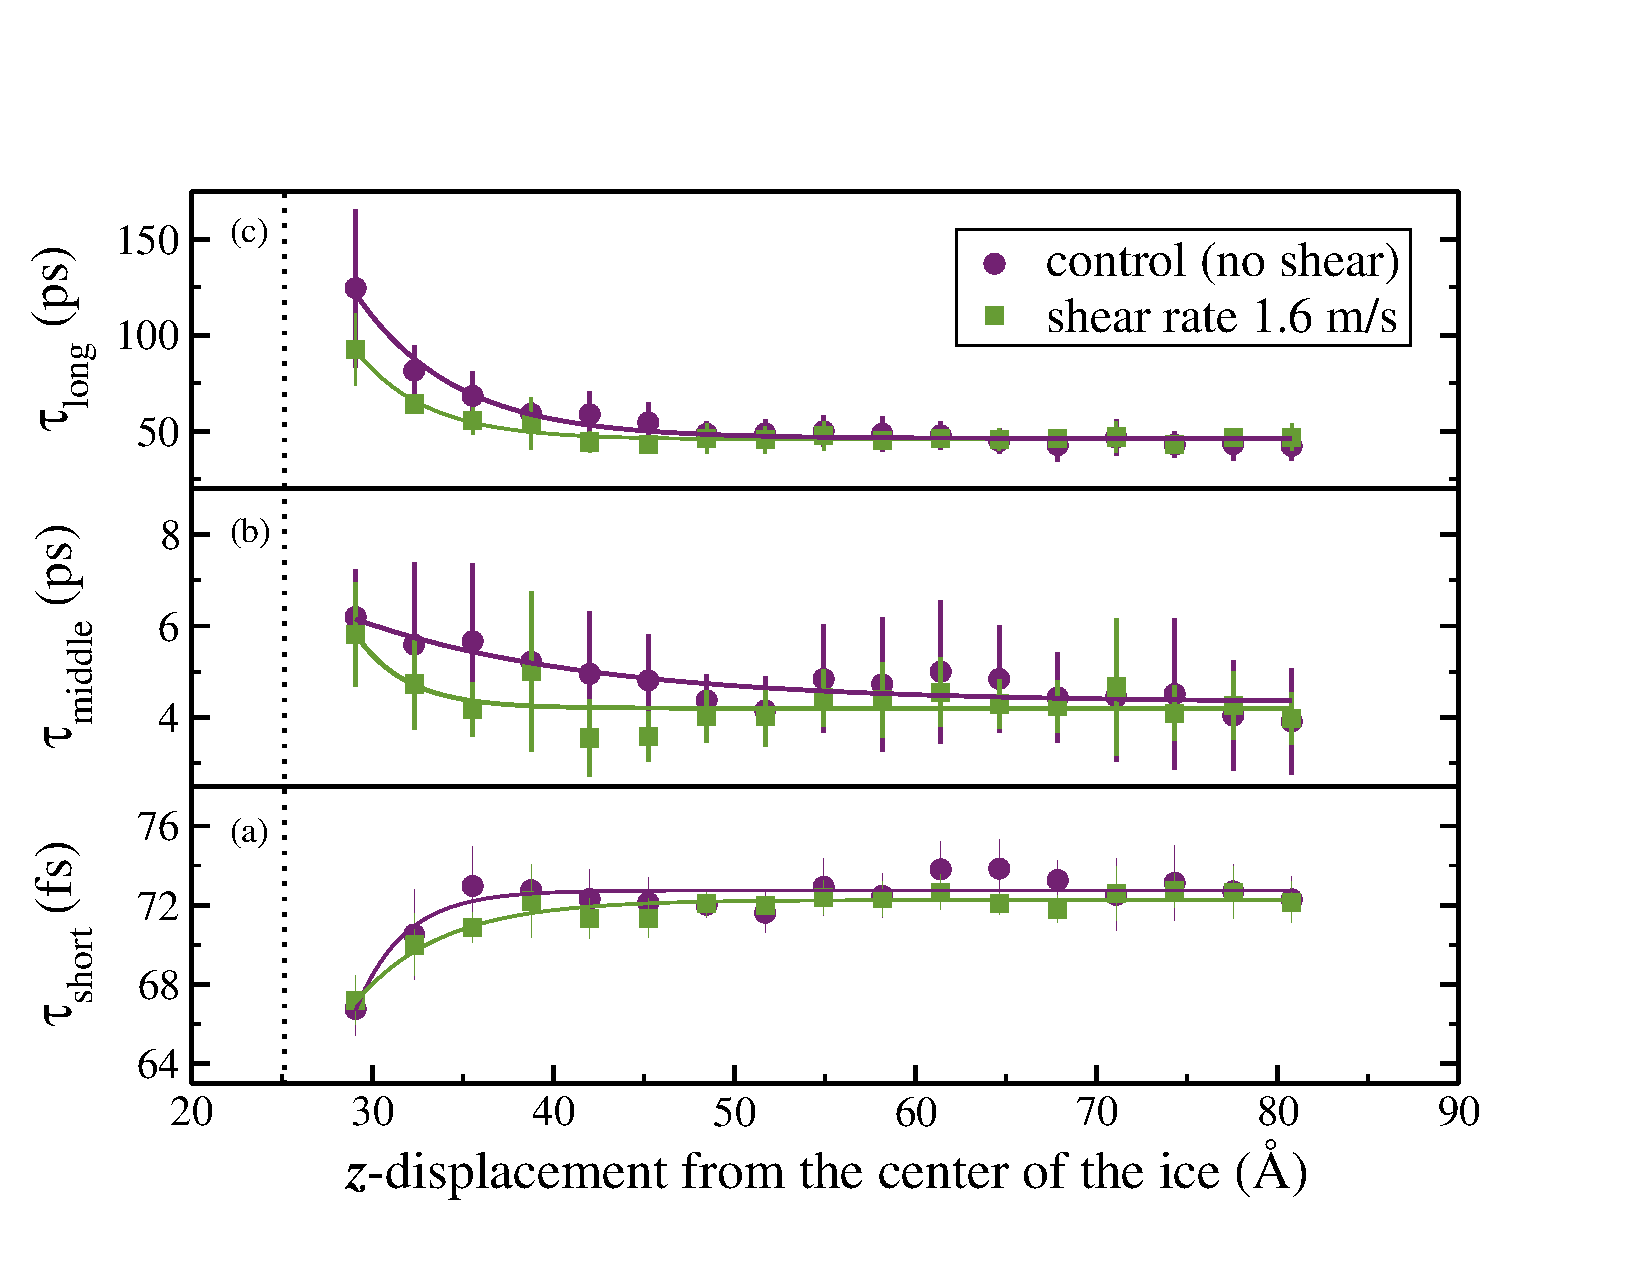
\includegraphics[width=\linewidth]{SP-orient}
\caption{\label{fig:SPorient} Decay constants for $C_2(z,t)$ at the secondary 
prism face. Panel descriptions match those in \ref{fig:PyrOrient}.}
\end{figure}


\begin{figure}
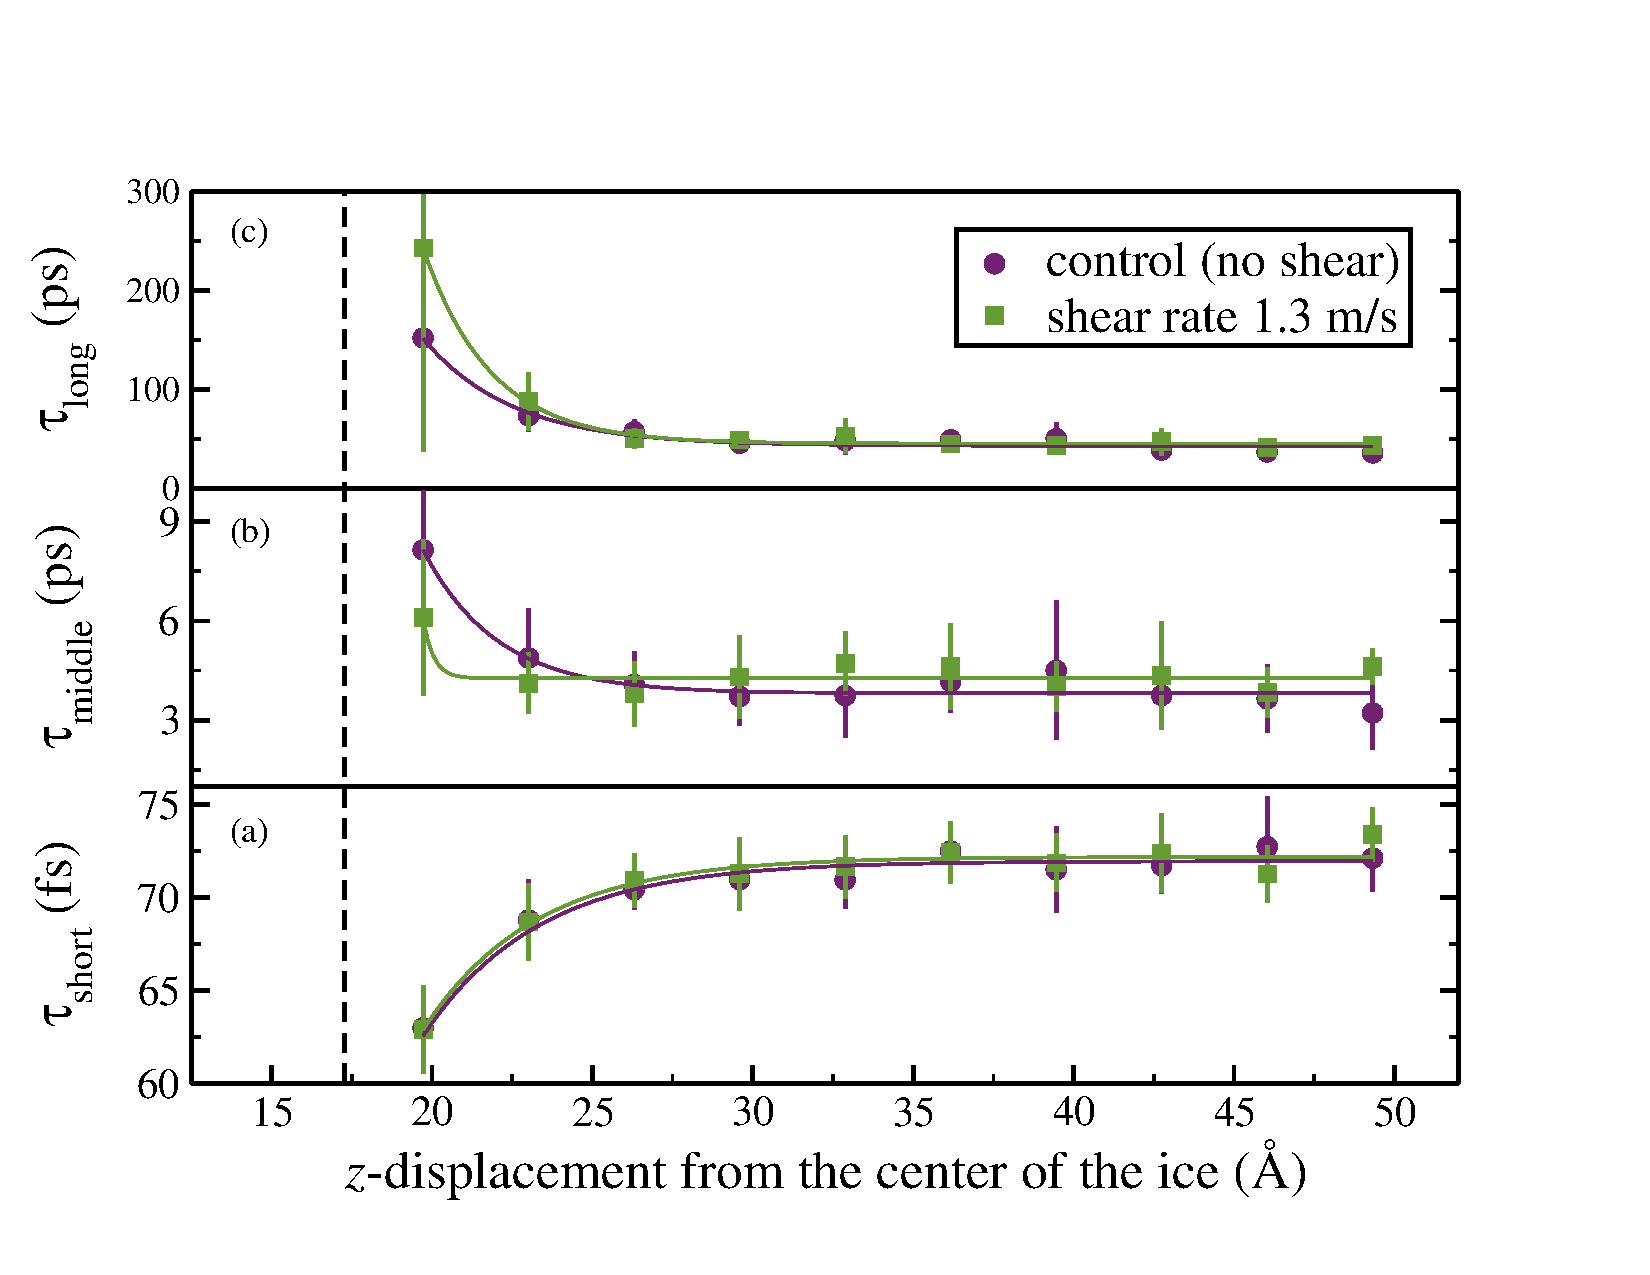
\includegraphics[width=\linewidth]{B-orient}
\caption{\label{fig:Borient} Decay constants for $C_2(z,t)$ at the basal face. Panel descriptions match those in \ref{fig:PyrOrient}.}
\end{figure}

\begin{figure}
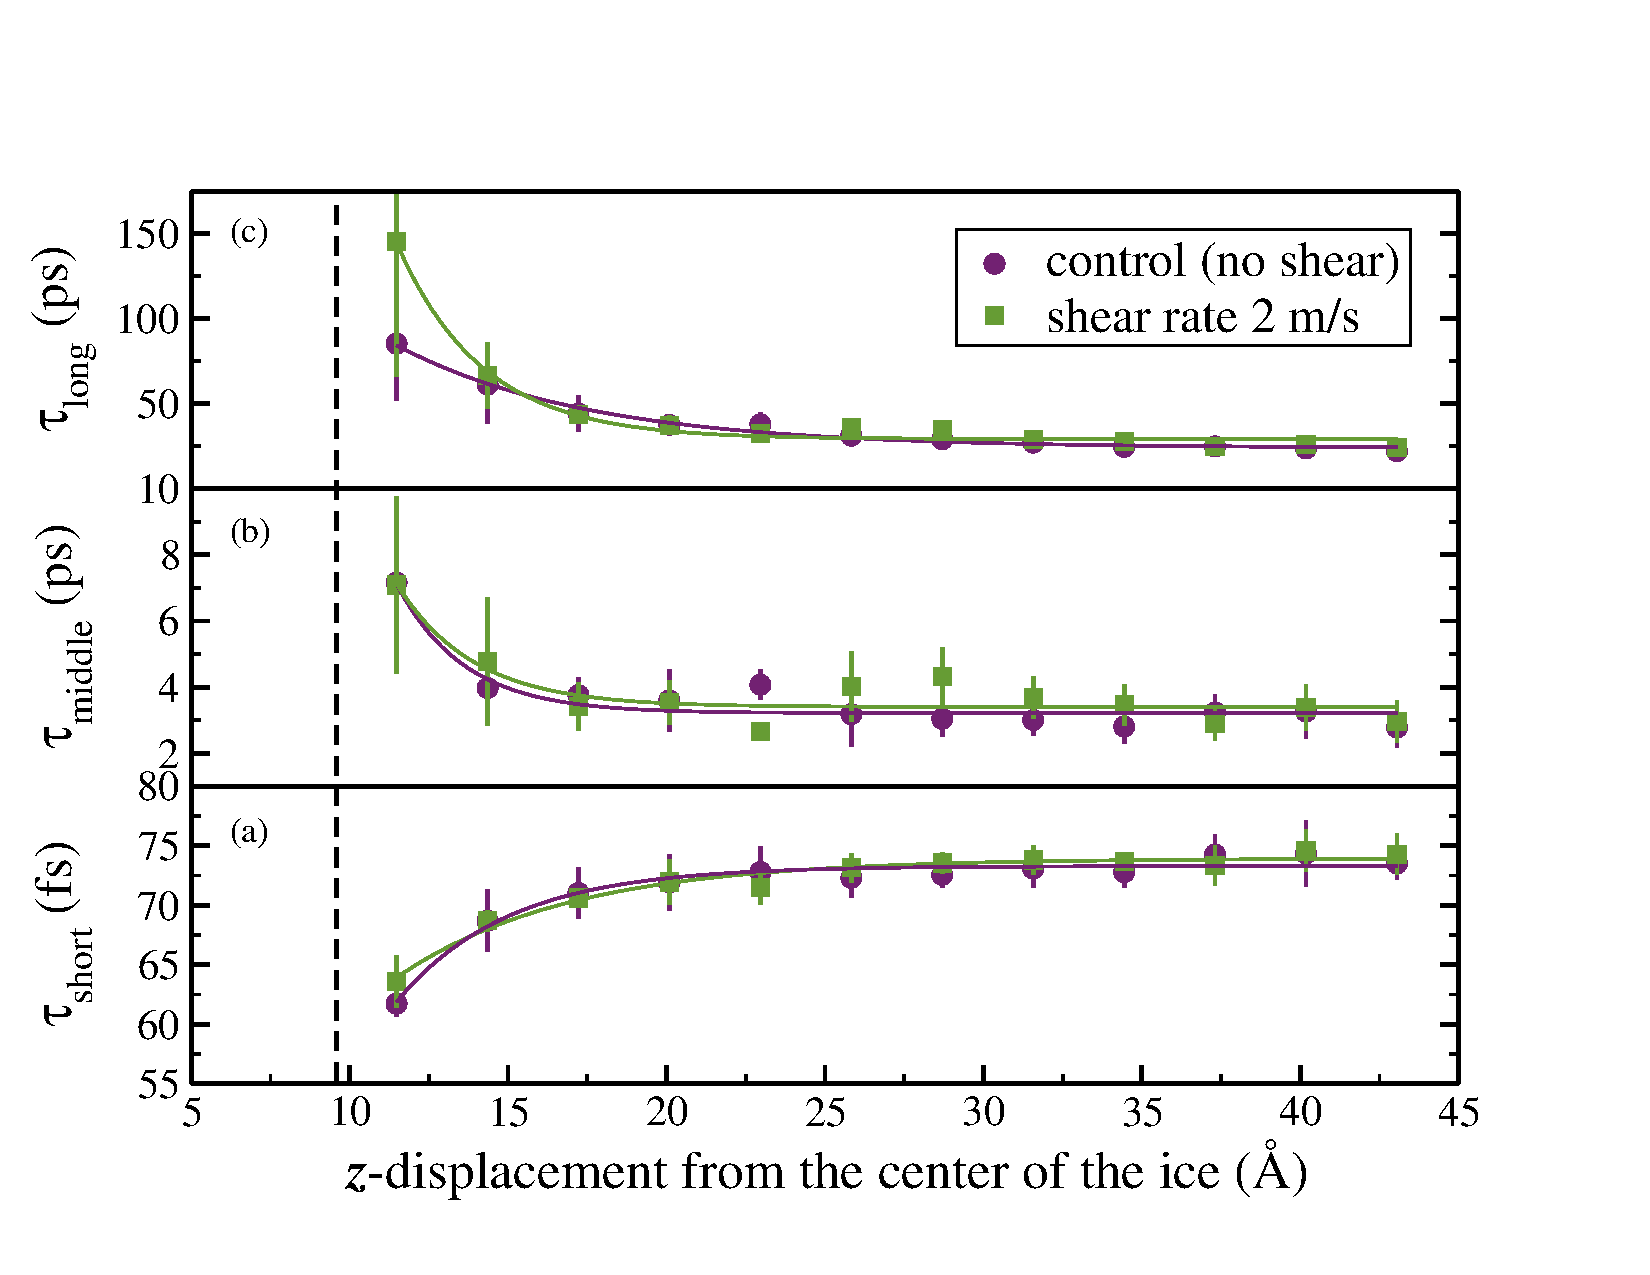
\includegraphics[width=\linewidth]{prismatic-orient}
\caption{\label{fig:Porient} Decay constants for $C_2(z,t)$ at the 
prismatic face. Panel descriptions match those in \ref{fig:PyrOrient}.}
\end{figure}


\end{document}
